\begin{tikzpicture}
  \node at (0,0) {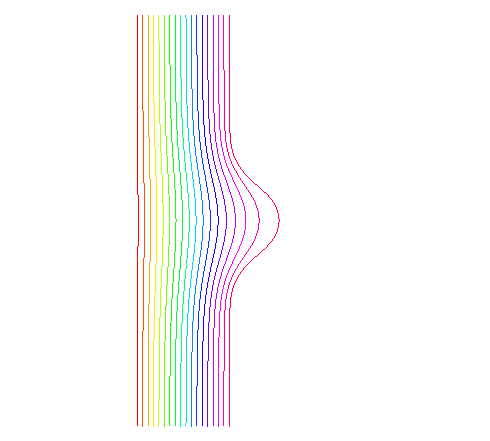
\includegraphics[scale=0.4]{gunfield.png}};
  \draw [fill=blue!40, radius=0.6]
    (-1.35,-1.95)
    -- ++(0,0.75)
    arc [start angle=0, end angle=90]
    -- ++(0,-1.75)
      coordinate [pos=0.1] (sample bottom)
    -- ++(-1,0)
    -- ++(0,-0.4)
    -- ++(1,0)
    arc [start angle=-90, end angle=0]
    -- cycle
  ;
  \draw [fill=blue!40, radius=0.6]
    (-1.35,1.4)
    -- ++(0,0.75)
    arc [start angle=0, end angle=90]
    -- ++(-1,0)
      node [pos=0.1,above] {$-V$}
    -- ++(0,-0.4)
    -- ++(1,0)
    -- ++(0,-1.75)
      coordinate [pos=0.9] (sample top)
    arc [start angle=-90, end angle=0]
    -- cycle
  ;
  \draw [fill=blue!40, radius=0.6]
    (0.15,-1.95)
    -- ++(0,0.75)
    arc [start angle=180, end angle=90]
    -- ++(0.4,0)
    -- ++(0,-2.15)
    -- ++(-0.4,0)
    arc [start angle=270, end angle=180]
    -- cycle
  ;
  \draw [fill=blue!40, radius=0.6]
    (0.15,1.4)
    -- ++(0,0.75)
    arc [start angle=180, end angle=90]
    -- ++(0.4,0)
      node [pos=0.1,above] {$0V$}
    -- ++(0,-2.15)
    -- ++(-0.4,0)
    arc [start angle=270, end angle=180]
    -- cycle
  ;
  \fill
   (sample top)
    -- (sample bottom)
      coordinate [pos=0.5] (source)
    -- ++(-0.2,0)
    -- ($(sample top) + (-0.2,0)$)
      node [pos=0.5, left]{Cathode}
    -- cycle
  ;
  \draw [green, <-, ultra thick]
    (source)
    -- ++(-52:4.2)
      node [black,below] {Laser}
  ;
\end{tikzpicture}

%TODO if time allows make wehnelt thinner
